\section{ConvLSTM}
Tradiční konvoluční neuronové sítě jsou výborným nástrojem pro zjišťování a práci s příznaky v prostorové doméně. Pokud je ale potřeba kromě prostorových dat nutné pracovat i s temporálními informacemi, musíme použít jiný nástroj. V takovém případě se nabízí použití ConvLSTM (Convolutional Long Short-Term Memory) sítě. Ta byla poprvé představena v roce 2015 v článku \cite{ConvLSTM}. Pro pochopení, jak ConvLSTM funguje, je ale nejdříve důležité pochopit, na jakém principu funguje tradiční LSTM síť, na které je ConvLSTM založená.

LSTM patří do skupiny rekurentních neuronových sítí (RNN), které slouží ke zpracování sekvenčních dat, kde existuje závislost aktuálního vstupu na předchozím.
Problémem použití klasických neuronový sítí na taková data je, že neuronová síť řeší každý vstup zvlášť a nemá žádný mechanismus, pomocí kterého by si dokázala spojit předchozí vstupy s těmi aktuálními.
Samozřejmě by se nabízela možnost dát na vstup neuronové sítě celou vstupní sekvenci, nebo alespoň její část, která se nachází bezprostředně před aktuálním vstupem, avšak to by znamenalo, že výsledná neuronová síť by musela být mnohem komplexnější, což by znamenalo větší nároky na výpočetní sílu a velikost trénovací množiny.
Rekurentní neuronové sítě tento problém řeší tím, že přidávají stavové proměnné, které ukládají informace o předchozích vstupech a jsou zpracovávány společně s aktuálním vstupem.

\begin{figure}[h!]
	\centering
	\subfloat[Architektura RNN]{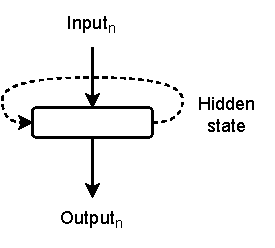
\includegraphics[width=0.3\textwidth]{Figures/solution/RNN_architecture.pdf}}
	\subfloat[Architektura RNN (rozvinutá)]{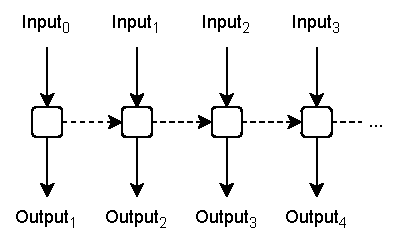
\includegraphics[width=0.4\textwidth]{Figures/solution/RNN_architecture_unrolled.pdf}}
	\caption{Diagram architektury RNN}
	\label{fig:RNN_architecture}
\end{figure}

Jak je patrné z obrázku \ref{fig:RNN_architecture}, tak pro každý vstup ve zpracovávané sekvenci je na základě tohoto vstupu a stavu stavové proměnné vzniklé zpracováním předchozího vstupu vytvořen výstup a nový stav skryté proměnné.
Jelikož je tato skrytá proměnná každým aktuálním vstupem měněna, dochází k tomu, že informace, která do ní byla zapsána při zpracování starších vstupů, ztrácí na významu a je překryta novějšími vstupy.
Rekurentní neuronové sítě z tohoto důvodu trpí problémy s dlouhodobější pamětí a jejich paměť je spíše krátkodobá.

LSTM se tento problém snaží vyřešit tak, že je specificky designovaná tak, aby více udržovala i dlouhodobější informace \cite{understaning_lstm}.
Samotný koncept LSTM již je celkem starý.
Poprvé byla síť LSTM představena v roce 1997 Hochreiterem a Schmidhuberem \cite{LSTM}.
Schéma LSTM je zobrazeno na obrázku \ref{fig:LSTM_architecture} a mnohým může připomínat strukturu logického obvodu.
Od toho se odvíjí i názvosloví, které tuto problematiku obklopuje, jelikož často mluví o branách.
Jak může být ze schématu patrné, tak LSTM má dvě stavové proměnné.

\begin{figure}[h!]
	\centering
	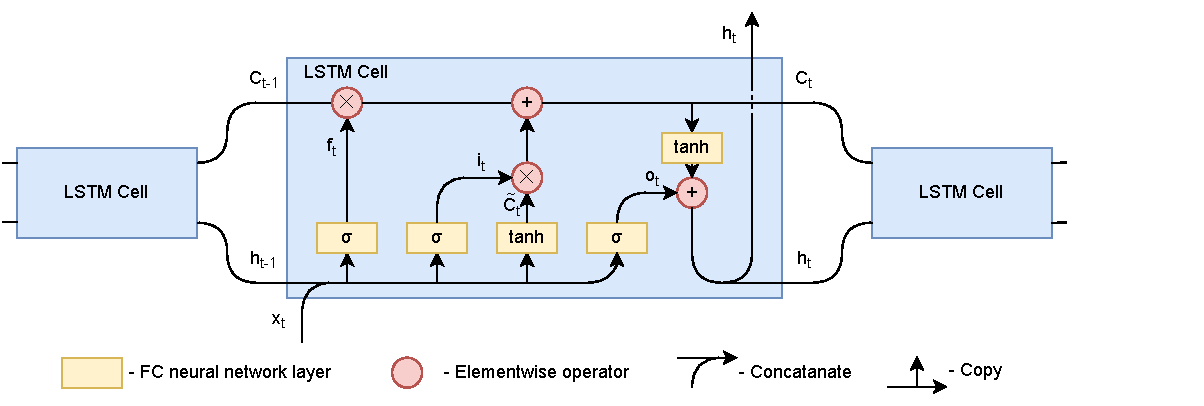
\includegraphics[width=\textwidth]{Figures/solution/LSTM_diagram.pdf}
	\caption{Struktura LSTM}
	\label{fig:LSTM_architecture}
\end{figure}



První z nich (procházející vrchní částí diagramu) slouží k ukládání dlouhodobých informací a často se nazývá stav buňky (cell state). Druhá z nich se nazývá skrytý stav (hidden state) a jedná se o paměť, se kterou LSTM buňka aktivně pracuje a na základě které rozhoduje, jak postupovat dále.
Postup vyhodnocování vstupních informací se dá rozdělit do několika kroků.

\begin{enumerate}

\item Na základě informací, které jsou obsaženy ve skrytém stavu a vstupním vektoru, je rozhodnuto, jaké informace ze stavu buňky budou ponechány a jaké budou zapomenuty.
O toto se stará tzv. zapomínací brána (Forget gate), tvořená plně propojenou vrstvou se sigmoidální aktivační funkcí.
Tato brána je následována Hadamardovým součinem výsledku této operace se stavem buňky.

Má-li být informace uložená v daném prvku stavu buňky zapomenuta, nastaví plně propojená vrstva hodnotu v odpovídajícím prvku na nulu.
V případě, že má být informace v prvku ponechána tak, jak je, bude ve výsledku FC vrstvy jednička.
Výsledek FC vrstvy samozřejmě může být jakékoliv číslo v intervalu \(<0;1>\) v závislosti na tom, jak moc má být informace zapomenuta a její vliv na další výpočet snížen.
Tuto bránu lze vyjádřit rovnicí \ref{eq:forget_gate}. 

\begin{equation}
f_t = \sigma(W_f \cdot [h_{t-1}, x_t] + b_f)
\label{eq:forget_gate}
\end{equation}


\item Následuje rozhodnutí o tom, jaké nové informace mají být ve stavu buňky uloženy.
Podobně jako v předchozím kroce jsou vstupní data společně se skrytým stavem dána na vstup vstupní brány (Input gate) tvořené FC vrstvou se sigmoidální aktivační funkcí, která určuje, jaká data mají být zapamatována.

\begin{equation}
i_t = \sigma(W_i \cdot [h_{t-1}, x_t] + b_i)
\label{eq:input_gate}
\end{equation}

Než jsou ale data do stavu buňky přidána, jsou předtím zpracována vstupní modulační branou (Input Modulation gate), která je také tvořena FC vrstvou, ale používá jako aktivační funkci hyperbolický tangens (\(\tanh\)).
Výsledek této operace je po složkách vynásoben s výsledkem vstupní brány a tento násobek je opět po jednotlivých složkách přičten k patřičným složkám ve stavu buňky.

\begin{equation}
\widetilde{C}_t = \tanh(W_{\widetilde{C}} \cdot [h_{t-1}, x_t] + b_{\widetilde{C}})
\label{eq:input_modulation_gate}
\end{equation}

Tímto jsou ukončeny veškeré modifikace stavu buňky \(C_t\) které by se daly vyjádřit rovnicí \ref{eq:cell_state_modification}, kde operátor \(\circ\) značí Hadamardův součin.

\begin{equation}
C_t = f_t \circ C_{t-1} + i_t \circ \widetilde{C}_t
\label{eq:cell_state_modification}
\end{equation}


\item Zbývá ještě poslední krok, a tím je vytvoření skrytého stavu buňky, který je zároveň i jejím výstupem.
Ten je vytvořen ze stavu buňky, avšak předtím, než jsou data dána na výstup jsou modifikována FC vrstvou s aktivační funkcí \(\tanh\).
Následně je ještě rozhodnuto, jaká data jsou na výstup propuštěna a v jaké míře.
K tomuto účelu slouží výstupní brána (Output gate), která je opět tvořena FC vrstvou se sigmoidální aktivační funkcí.
Na vstupu tato brána bere vstupní data společně se skrytým stavem a na jejich základě rozhodne o tom, jaké informace ze stavu buňky budou propuštěny dále.

\begin{equation}
o_t = \sigma(W_o \cdot [h_{t-1}, x_t] + b_o)
\label{eq:output_gate}
\end{equation}

Výpočet výstupu LSTM buňky a jejího skrytého stavu lze tedy vyjádřit rovnicí \ref{eq:output}.

\begin{equation}
h_t = o_t \circ \tanh(C_t)
\label{eq:output}
\end{equation}

\end{enumerate}

V literatuře se dá narazit i na verzi LSTM, která využívá tzv. špehýrková spojení (peephole connections), která byla přidána do LSTM architektury Gersem a Schidhuberem v roce 2000. \cite{PeepLSTM}
Tato spojení způsobují, že ke vstupu všech bran, které mají sigmoidální aktivační funkci, je přidán i stav buňky. U zapomínácí a vstupní brány jde o \(h_{t-1}\), neboli stav buňky před jakýmikoliv modifikacemi, zatímco u brány výstupní je použit již modifikovaný stav  \(h_{t}\).
Brány tedy rozhodují nejen na základě aktuálního vstupu a skrytého stavu buňky, ale i podle obsahu stavu buňky.
Vzorce \ref{eq:forget_gate} a \ref{eq:input_gate} by tedy šly v tomto případě napsat podle vzoru \( A_t = \sigma(W_A \cdot [h_{t-1}, x_t, C_{t-1}] + b_A) \), kde za \(A\) dosadíme \(f\) nebo \(i\), a vzorec \ref{eq:output_gate} by vypadal \( o_t = \sigma(W_o \cdot [h_{t-1}, x_t, C_{t}] + b_o) \).


Konvoluční LSTM vrstvy ConvLSTM spojují výhody konvolučních vrstev, které jsou skvělé pro zpracování prostorových informací a LSTM vrstev, které dobře zpracovávají temporální informace, a proto jsou jedním z nástrojů, které je možné použít pro práci s časoprostorovými daty.

Na rozdíl od klasické LSTM vrstvy rozhoduje ConvLSTM o novém stavu buňky nejen na základě jejího vstupu a jejích skrytých stav a také na základě vstupů a skrytých stavů jejích sousedů.
Vstupy, výstupy a skryté stavy jsou z tohoto důvodu u ConvLSTM reprezentovány pomocí 3D tenzorů, jejichž poslední dvě dimenze jsou dimenze prostorové.
Na tyto tenzor jsou následně použity konvoluční operace pro výpočet nového stavu buňky a skrytého stavu. Ekvivalenty vzorců popisujících jednotlivé brány v LSTM tedy vypadají následovně.

\begin{equation}
f_t = \sigma(W_{f} * [x_t, h_{t-1}] + b_f)
\label{eq:ConvLSTM_forget_gate}
\end{equation}

\begin{equation}
i_t = \sigma(W_{i} * [x_t, h_{t-1}] + b_i)
\label{eq:ConvLSTM_input_gate}
\end{equation}

\begin{equation}
\widetilde{C}_t = \tanh(W_{c} * x_t + b_c)
\label{eq:ConvLSTM_input_modulation_gate}
\end{equation}

\begin{equation}
o_t = \sigma(W_{o} * [x_t, h_{t-1}] + b_o)
\label{eq:ConvLSTM_output_gate}
\end{equation}

I u ConvLSTM je možné se setkat s verzí obsahující špehýrková spojení.
V tomto případě ale není stav buňky pouze konkatenován se vstupem a skrytým stavem před tím, než je na ně použita konvoluce.
Místo toho je k nim přidán až po provedení této operace a místo konvoluce je svými vahami upraven pouze Hadamardovým součinem.

Aby šel vstup, stav buňky a skrytý stav jednoduše konkatenovat, musí mít stejné prostorové rozměry.
Z tohoto důvodu musí být velikost obrázků, které bude síť zpracovávat, známa předem, jelikož skryté stavy ConvLSTM buňky musí být inicializovány na správnou velikost.

Změnou velikosti konvoluční masky se dá měnit na jak rychle pohybující se objekty bude výsledná síť citlivá.
Je jasné, že maska o velikosti 3x3 nebude efektivní pro zpracování objektu, který překoná během jediného snímku polovinu celého scény, která má na snímku stovky pixelů.
Lidé se však moc rychle nepohybují a v případě, kdy jsou snímání kamerou se snímací frekvencí 30Hz, je tento pohyb o to menší. Síť ResNet, která je použita bezprostředně před ConvLSTM vrstvami navíc zmenšuje prostorové dimenze vstupních vektorů, tudíž v tomto případě je maska o velikosti 3x3 dostatečná.
V navržené síti jsou proto použity 2 po sobě jdoucí ConvLSTM vrstvy s velikostí konvoluce 3x3, které následují po extrakci prostorových příznaků pomocí sítě ResNet.
Dvě vrstvy jsou použity z toho důvodu, že v případě, že je v síti použito více ConvLSTM vrtstev, je taková síť schopná ze vstupní sekvence extrahovat složitější časoprostorové příznaky.

\endinput